\subsection{Disk performance}

\subsubsection{HDD}

We can calculate some performance metrics related to the types of delay of HDD (page \pageref{four types of hdd delay}).
\begin{itemize}
    \item \definition{Full Rotation Delay} $R$ is:
    \begin{equation}
        R = \dfrac{1}{\texttt{DiskRPM}}
    \end{equation}
    And in seconds:
    \begin{equation}
        R_{\text{sec}} = 60 \times R
    \end{equation}
    From the $R_{\text{sec}}$ we can also calculate the \definition{total rotation average}:
    \begin{equation}
        T_{\text{rotation AVG}} = \dfrac{R_{\text{sec}}}{2}
    \end{equation}

    \item \definition{Seek Time}, the \textbf{time to move the head to a different track}, which is divided into several phases:
    \begin{itemize}
        \item Acceleration
        \item Coasting (constant speed)
        \item Deceleration
        \item Settling
    \end{itemize}
    The $T_{\text{seek}}$ modelling considers a linear dependency with the distance. Also, the \definition{seek average} is:
    \begin{equation}
        T_{\text{seek AVG}} = \dfrac{T_{\text{seek MAX}}}{3}
    \end{equation}

    \item \definition{Transfer time}. It is the \textbf{time that data is either read from or written to the surface}. It \textbf{includes} the time the \textbf{head needs to pass on the sectors} and the \textbf{I/O transfer}:
    \begin{equation}
        T_{\text{transfer}} = \dfrac{\text{R/W of a sector}}{\text{Data transfer rate}}
    \end{equation}
    The \definition{Controller Overhead} is the \textbf{buffer management} (data transfer) and \textbf{interrupt sending time}.

    Transfer time and Controller Overhead are together because they are required to calculate some interesting metrics.
    \begin{itemize}
        \item \definition{Service Time} $T_{\text{I/O}}$
        \begin{equation}
            T_{\text{I/O}} = T_{\text{seek}} + T_{\text{rotation}} + T_{\text{transfer}} + T_{\text{overhead}}
        \end{equation}

        \item \definition{Response Time}
        \begin{equation}
            T_{\text{queue}} + T_{\text{I/O}}
        \end{equation}
        Where $T_{\text{queue}}$ depends on queue-length, resource utilization, mean and variance of disk service time and request arrival distribution.
    \end{itemize}
    \newpage
    \begin{figure}[!htp]
        \centering
        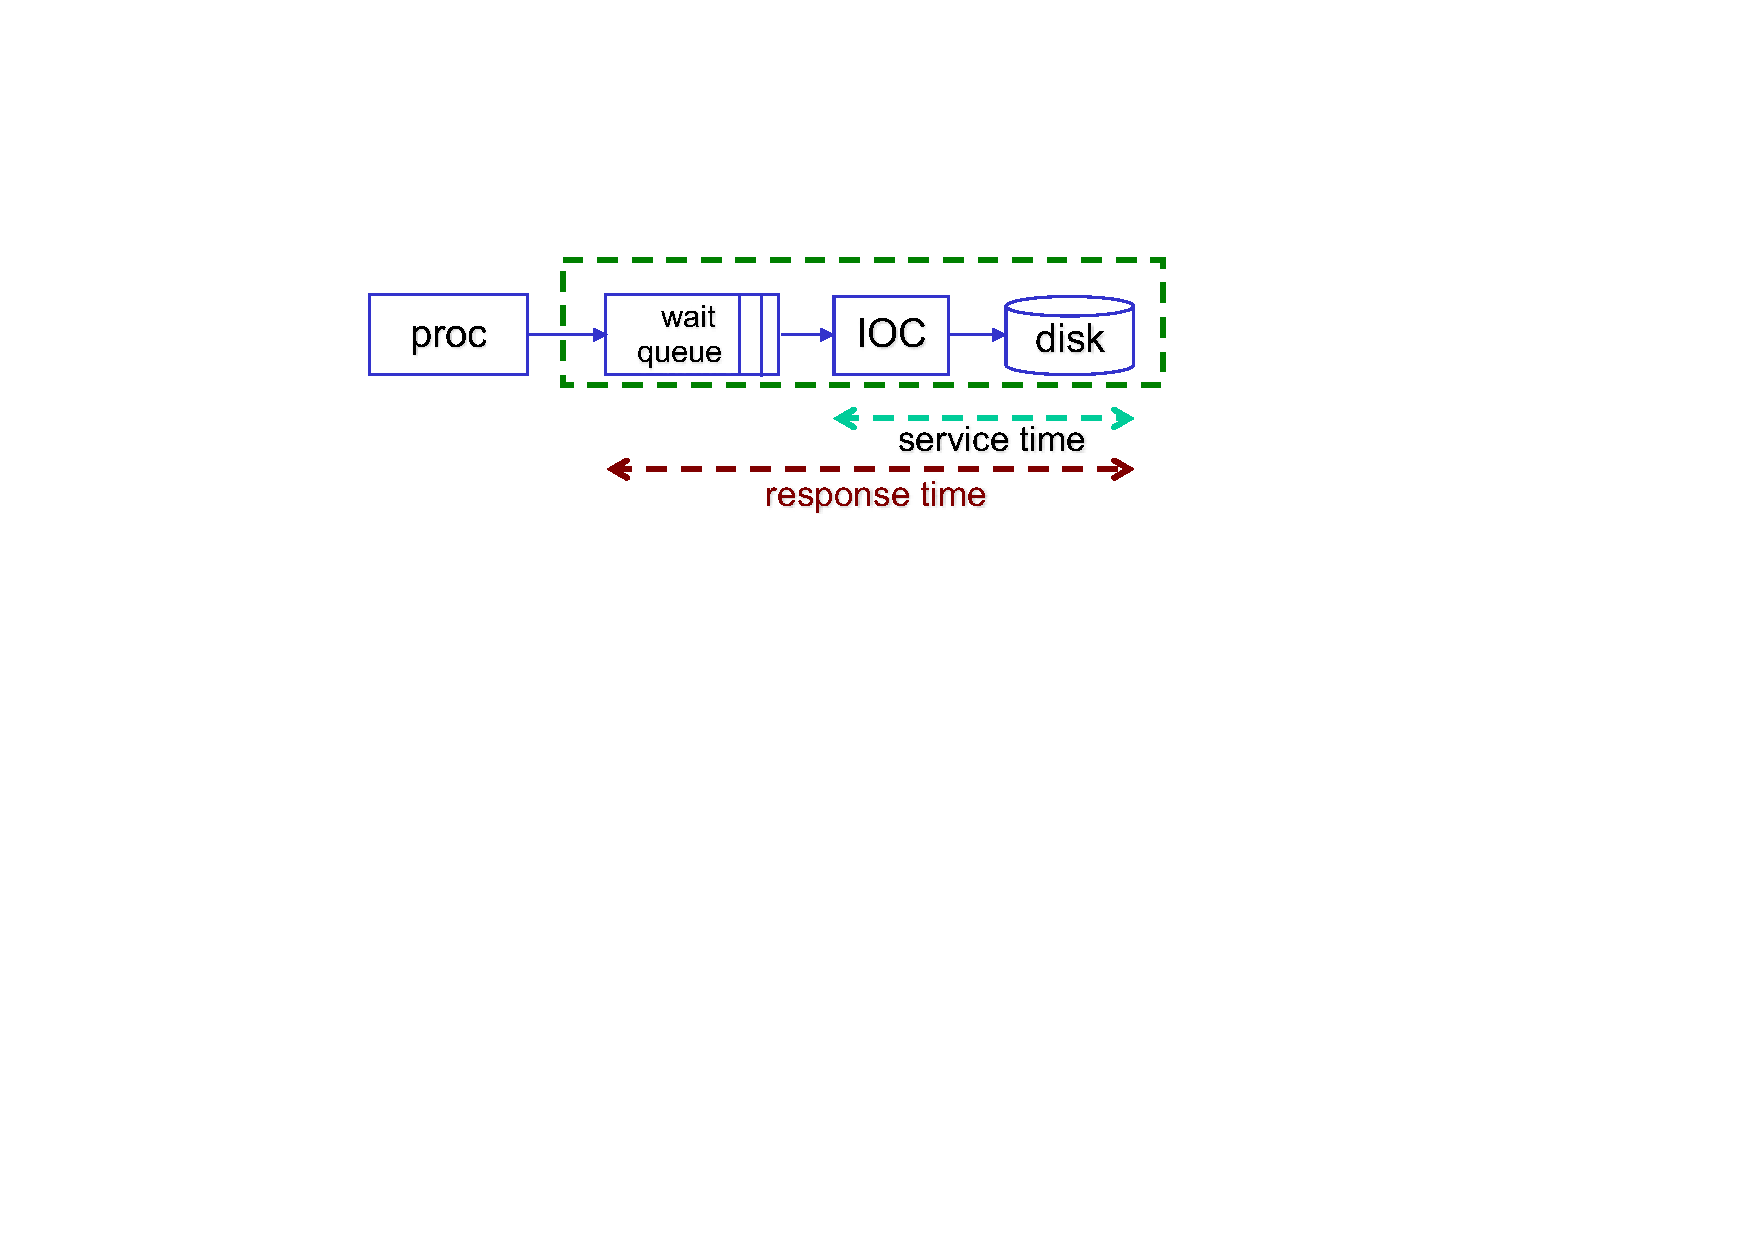
\includegraphics[width=.7\textwidth]{img/performance-hdd-1.pdf}
        \caption{Service and response time.}
    \end{figure}
\end{itemize}

\begin{exercisebox}[: mean service time of an I/O operation]\label{exercise: mean service time of an I/O operation}
    The data of the exercise are:
    \begin{itemize}
        \item Read/Write of a sector of $512$ bytes ($0.5$ KB)
        \item Data \underline{transfer} rate: $50$ MB/sec
        \item \underline{Rotation} speed: $10000$ RPM (Round Per Minute)
        \item Mean \underline{seek} time: $6$ ms
        \item Overhead \underline{Controller}: $0.2$ ms
    \end{itemize}
    To calculate the \emph{service time} $T_{\text{I/O}}$, we need the following information:
    \begin{itemize}
        \item $T_{\text{seek}}$, which we already have, and it is $6$ ms.
        \item $T_{\text{rotation}}$
        \item $T_{\text{transfer}}$
        \item $T_{\text{overhead}}$, which we already have, and it is $0.2$ ms.
    \end{itemize}
    We also know the rotation and transfer information, but we want to know the \emph{mean} service time. Then we calculate the total rotation average $T_{\text{rotation AVG}}$:
    \begin{equation*}
        \begin{array}{rcl}
            R &=& \dfrac{1}{\texttt{DiskRPM}} = \dfrac{1}{10000} = 0.0001 \\ [1em]
            R_{\text{sec}} &=& 60 \cdot R = 60 \cdot 0.0001 = 0.006 \text{ seconds} \\ [1em]
            T_{\text{rotation AVG}} &=& \dfrac{R_{\text{sec}}}{2} = \dfrac{0.006}{2} = 0.003 \text{ seconds} = 3 \text{ ms}
        \end{array}
    \end{equation*}
    Finally, the transfer time is easy to calculate because we have the R/W of a sector and the data transfer rate. First we do a conversions from megabytes to kilobytes:
    \begin{equation*}
        \begin{array}{rcl}
            \text{Data transfer rate: }&& 50 \text{ MB/sec} \\ [1em] 
            &=& 50 \cdot 1024 \text{ KB/sec} \\ [1em] 
            &=& 51200 \text{ KB/sec} \\ [1em]
            T_{\text{transfer}} &=& \dfrac{0.5 \text{ KB/sec}}{51200 \text{ KB/sec}} \\ [1em]
            &=& 0.000009765625 \text{ sec } \cdot 1000 \\ [1em]
            &=& 0.009765625 \text{ ms } \approx 0.01 \text{ ms}
        \end{array}
    \end{equation*}
    The exercise can be completed by calculating the mean I/O service time required:
    \begin{equation*}
        \begin{array}{rcl}
            T_{\text{I/O}} &=& T_{\text{seek}} + T_{\text{rotation}} + T_{\text{transfer}} + T_{\text{overhead}} \\ [.8em]
            T_{\text{I/O}} &=& 6 + 3 + 0.01 + 0.2 = 9.21 \text{ ms}
        \end{array}
    \end{equation*}
\end{exercisebox}

\noindent
The previous service time is supposed to be only for very \textbf{pessimistic cases} where \textbf{sectors are fragmented on the disk in the worst possible way}. This can happen because the files are tiny (each file is contained in one block) or the disk is externally fragmented.

\highspace
Thus, each access to a sector requires to pay rotational latency and seek time.
This is not the case in many circumstances because the files are larger than one block and stored contiguously.

\highspace
We can measure the \definition{Data Locality $DL$} of a disk as the \textbf{percentage of blocks that do not need seek or rotational latency to be found}.

\highspace
Thanks to the Data Locality, it is possible to calculate the \definition{Average Service Time}:
\begin{equation}
    T_{\text{I/O AVG}} = \left(1 - DL\right) \cdot \left(T_{\text{seek}} + T_{\text{rotation}}\right) + T_{\text{transfer}} + T_{\text{controller}}
\end{equation}


\begin{exercisebox}[: data locality]
    The data of the exercise are:
    \begin{itemize}
        \item Read/Write of a sector of $512$ bytes ($0.5$ KB)
        \item \underline{Data Locality}: $DL = 75\%$
        \item Data \underline{transfer} rate: $50$ MB/sec
        \item \underline{Rotation} speed: $10000$ RPM (Round Per Minute)
        \item Mean \underline{seek} time: $6$ ms
        \item Overhead \underline{Controller}: $0.2$ ms
    \end{itemize}
    Since the Data Locality is $75\%$, only $25\%$ of the operations are affected by the DL:
    \begin{equation*}
        \left(1-DL\right) = \left(1 - 0.75\right) = 0.25
    \end{equation*}
    See the exercise on page \pageref{exercise: mean service time of an I/O operation} to understand the values of $T_{\text{seek}}$, $T_{\text{rotation}}$, $T_{\text{transfer}}$ and $T_{\text{overhead}}$:
    \begin{itemize}
        \item $T_{\text{seek}} = 6$
        \item $T_{\text{rotation}} = 3$
        \item $T_{\text{transfer}} = 0.01$
        \item $T_{\text{overhead}} = 0.2$
    \end{itemize}
    Finally the average time for read/write a sector of $0.5$ KB with a DL of $75\%$ is:
    \begin{equation*}
        \begin{array}{rcl}
            T_{\text{I/O AVG}} &=& 0.25 \cdot \left(6 + 3\right) + 0.01 + 0.2 \\ [1em]
            &=& 0.25 \cdot 9 + 0.21 \\ [1em]
            &=& 2.46 \text{ ms}
        \end{array}
    \end{equation*}
\end{exercisebox}

\begin{exercisebox}[: influence of \dquotes{not optimal} data allocation]
    The data of the exercise are:
    \begin{itemize}
        \item $10$ blocks of $1/10$ MB for each block ($10$ blocks of $1/10$ MB \dquotes{not well} distributed on disk)
        \item $T_{\text{seek}} = 6$ ms
        \item $T_{\text{rotation AVG}} = 3$ ms
        \item Data transfer rate: $50$ MB/sec
    \end{itemize}
    In the exercise you were asked to calculate the time taken to transfer a 1 MB file with 100\% and 0\% data locality:
    \begin{itemize}
        \item Data Locality equals to 100\%:
        \begin{itemize}
            \item An initial seek ($6$ ms)
            \item A total rotation average ($3$ ms)
            \item Now it's possible to do the 1MB global transfer directly because there are no blocks to seek or rotation latency:
            \begin{equation*}
                \text{1 MB of 50 MB} = \dfrac{1}{50} = 0.02 \text{ seconds } \cdot 1000 = 20 \text{ ms}
            \end{equation*}
            \item The total time is:
            \begin{equation*}
                T = 6 + 3 + 20 = 29 \text{ ms}
            \end{equation*}
        \end{itemize}

        \newpage
        \item Data Locality equals to 0\%:
        \begin{itemize}
            \item An initial seek ($6$ ms)
            \item A total rotation average ($3$ ms)
            \item In this case, it's not possible to do a global transfer directly, because each block is affected by the seek or rotation latency. Then we have to transfer block by block and calculate the delay:
            \begin{equation*}
                \text{1 MB of 10 MB} = \dfrac{1}{10} = 0.1 \text{ seconds } \cdot 1000 = 100 \text{ ms}
            \end{equation*}
            \item The total time is:
            \begin{equation*}
                T = \left(6 + 3 + 2\right) \cdot 10 = 110 \text{ ms}
            \end{equation*}
            Where $10$ is the number of blocks.
        \end{itemize}
    \end{itemize}
    Note: the controller times is not considered.
\end{exercisebox}
